
\section{Análisis}

En esta sección se muestra el análisis de las técnicas empleadas para el reconocimiento de voz, la implementación y diversas pruebas para la elección del sistema propuesto.

\subsection{Del reconocimiento de voz}

	El análisis y elección de técnicas para la etapa de reconocimiento se hacen con base al estado del arte presentado en este documento.
	
	Como se vio en la sección \ref{sub:sr} los artículos \cite{A30}, \cite{A31}, \cite{A6} y \cite{A7} mencionan explicitamente algunas de las características de la voz para que esté adecuada a la etapa de reconocimiento. En general el pre-procesamiento de la señal de voz se lleva a cabo de acuerdo al bloque mostrado en la Figura \ref{fig:ana:prepro}.
	
		\begin{figure}[H]
			\centering
			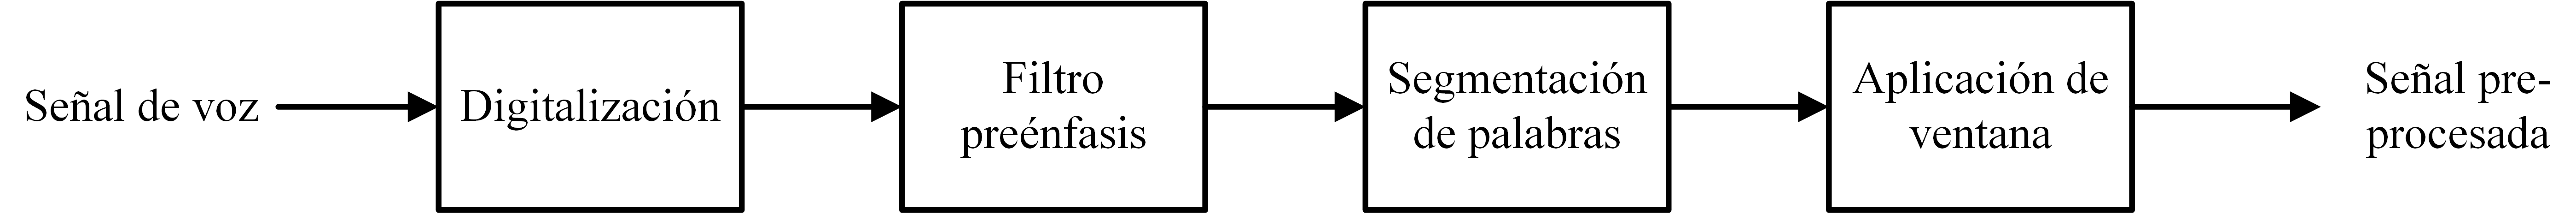
\includegraphics[width=1\linewidth]{figures/analisispreproce}
			\caption{Diagrama de la etapa de pre-procesamiento.}
			\label{fig:ana:prepro}
		\end{figure}
		
	De acuerdo a la Figura \ref{fig:ana:prepro} obtenemos las siguientes etapas a seguir:
	
	\subsubsection*{Digitalización}
	
	La digitalización es el primer proceso que se llevará a cabo y será la conversión de la señal de voz analógica a digital, esto a través del micrófono del dispositivo móvil. Para este proceso se decide utilizar una frecuencia de muestreo de 8 kHz y un tamaño de muestra de 8 bits, esto con el fin de optimizar los recursos del teléfono móvil. Dados los alcances presentados la duración máxima de la grabación de voz será de 10 segundos, por lo que la memoria máxima que ocupará un mensaje de voz será de $memoria=(8000\frac{muestras}{segundo}\cdot 10 segundos\cdot 8\frac{bits}{muestra}=640000 bits = 78.125 kB$, por lo que en una conectividad 4G con una velocidad de subida de 50Mbps, la señal de voz con mayor duración tardará 12.8 ms en ser enviada al servidor.
	
	\subsubsection*{Preénfasis}
	
	Como se vio en la sección del estado del arte, diversos artículos aplican el filtro preénfasis para resaltar características de la señal de voz, para esto se usa la fórmula $\hat{s}(n)=s(n)-a\cdot s(n-1)$, el valor de $a$ que se usará es el propuesto en \cite{A6} que es de $a=0.95$, en la Figura \ref{fig:ana:preenfasis} se muestra la aplicación del filtro a una señal de voz, así como también su espectro correspondiente, en éstos podemos observar cómo el espectro correspondiente a la señal filtrada se ve aplanado, de esta forma se pueden apreciar con mayor medida los formantes de la señal, para este caso, el interlocutor es una mujer de 22 años, y de acuerdo a la teoría, la frecuencia fundamental para las mujeres se encuentra entre los 200 y 250 Hz, en este caso lo podemos ubicar en los 200 Hz.
	
		\begin{figure}[H]
			\centering
			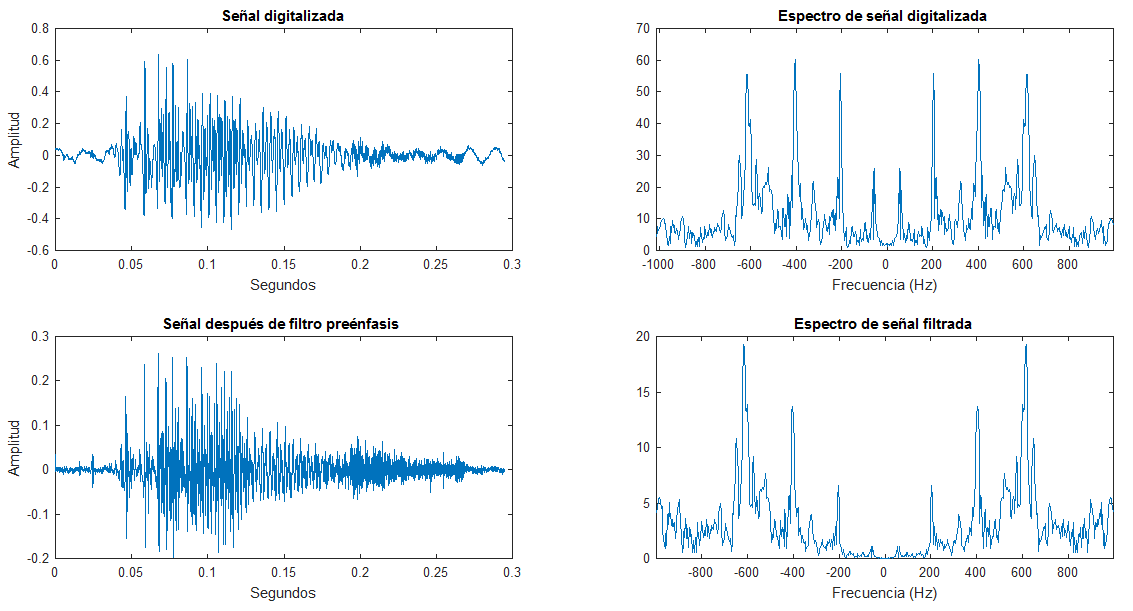
\includegraphics[width=1\linewidth]{figures/preenfasis}
			\caption{Aplicación del filtro de preénfasis.}
			\label{fig:ana:preenfasis}
		\end{figure}
	
	\subsubsection*{Detección de inicio y final de las palabras}
	
	Para la detección de bordes de palabras aisladas Rabiner en \cite{Rabiner1975} propone un algoritmo que hace uso de la energía de la señal y la tasa de cruces por cero y \cite{A31} por otro lado, propone el uso de la energía de la señal y la tasa de cruces por cero en tiempo corto, además de dos características en el dominio de la frecuencia, que son el centroide y flujo espectral, debido a los resultados de 96.25\% de éxitos en la segmentación de \cite{A31} se haría uso de este algoritmo de umbral dinámico para llevar a cabo la segmentación de las palabras de la frase a reconocer, sin embargo, tomando en cuenta que el tiempo de respuesta del sistema debe ser adecuada para llevar a cabo una conversación fluida y con esto que la experiencia de usuario no se vea afectada se decide hacer uso de la energía y tasa de cruces por cero para llevar a cabo la detección de bordes de la palabra y de esta forma llevar a cabo su separación. 
	
	\subsubsection*{Segmentación y aplicación de la ventana}
	
	La segmentación se lleva a cabo para que la señal de voz sea tratada como una señal estacionaria, la longitud del segmento que se propone en \cite{A6}, que corresponde a 45 ms del segmento con un espaciado de 15 ms y un traslape de 30 ms presentan buenos resultados, sin embargo, dados los tiempos de respuesta, esto implica llevar un mayor procesamiento, por lo que se proponen segmentos de 40 ms de duración y un traslape del 50\%. La ventana que será aplicada es la ventana de Hamming, esto debido a que la mayoría de los artículos la usa y como se mencionó en el marco teórico es la ventana que guarda la mejor relación de lóbulo central y laterales. En la Figura \ref{fig:ana:windowing} se puede observar uno de estos segmentos de la señal de voz con la ventana Hamming aplicada, es apreciable el amortiguamiento que genera la ventana y la periodicidad que obtiene la señal gracias a la segmentación.
	
	 \begin{figure}[H]
			\centering
			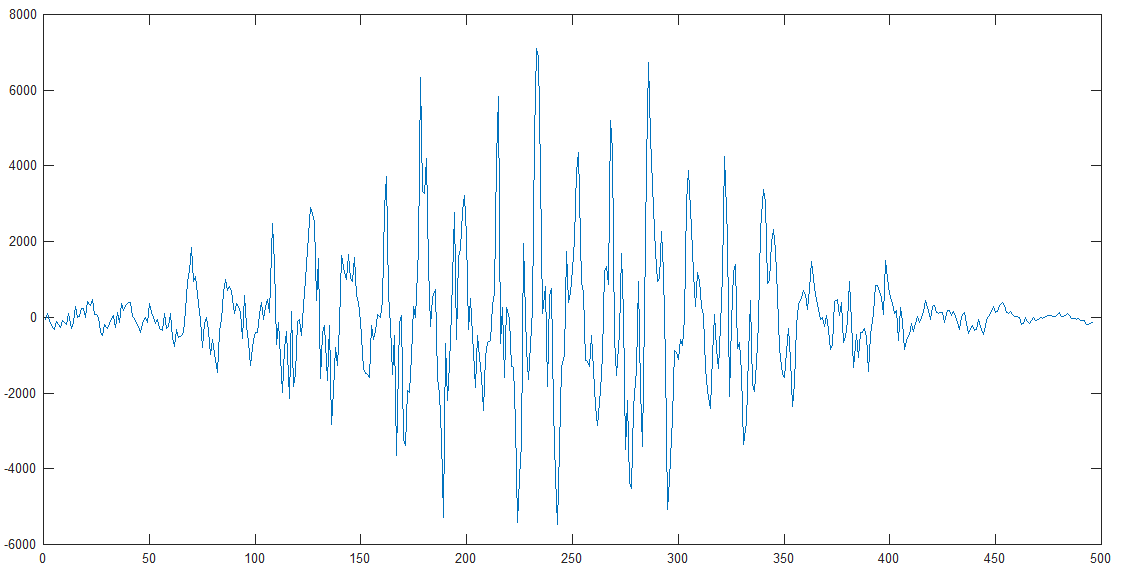
\includegraphics[width=0.8\linewidth]{figures/windowing}
			\caption{Segmentación y ventaneo de la señal de voz.}
			\label{fig:ana:windowing}
	\end{figure}
	
	\subsubsection*{Extracción de características}
	
	La siguiente fase es la extracción de características, de acuerdo a \cite{A1} el estado del arte de extracción de características es la técnica MFCC ya que se basa en el sistema auditivo humano y dados los resultados experimentales de eficiencia del 80\% se ha decidido que es la técnica que se usará en el sistema. De acuerdo a la literatura el proceso de extracción de características se realiza de acuerdo a las siguientes técnicas de procesamiento:
	
	\begin{itemize}
	\item	Filtro preénfasis
	\item	Entramado y ventaneo
	\item	Transformada de Fourier
	\item	Banco de filtros de Mel
	\item	Logaritmo de la señal transformada
	\item	Transformada del coseno discreto
	\end{itemize}
	
	En la Figura \ref{fig:ana:HolaRecorte} se muestran los coeficientes cepstrales en la escala de Mel de la palabra \textit{Hola}, en la gráfica superior se muestran los coeficientes correspondientes a la grabación completa y en la inferior a la grabación recortada. De acuerdo a la teoría, el primer coeficiente de cada segmento representa la energía de ese segmento, en la gráfica superior podemos observar la importancia de este coeficiente, pues su valor es mayor en la región en la que se genera la voz y en los silencios este coeficiente tiene un valor menor, así, se puede hacer uso de este coeficiente para llevar a cabo la segmentación de las palabras como se puede ver en la gráfica inferior que representa a la realización de la palabra y observamos que el coeficiente cero tiene mayor intensidad en cada segmento.
	
	 \begin{figure}[H]
			\centering
			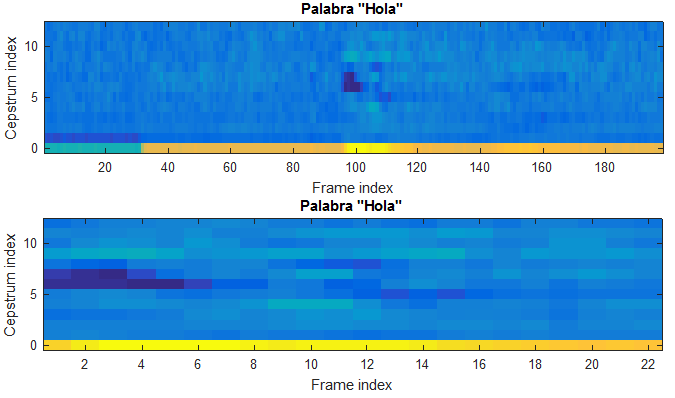
\includegraphics[width=0.8\linewidth]{figures/mfccHolaRecorte}
			\caption{Coeficientes en la escala de Mel, palabra ``Hola''.}
			\label{fig:ana:HolaRecorte}
	\end{figure}
	
	En la Figuras \ref{fig:ana:mfccHola} y \ref{fig:ana:mfccTren} se muestran los coeficientes cepstrales en la escala de Mel de las palabras \textit{Hola} y \textit{Tren} pronunciadas por diferentes personas. Como se puede observar, entre los coeficientes de la misma palabra existen ciertas similitudes como la intensidad en los segmentos, mientras que entre los diferentes interlocutores se observan ciertas características, por ejemplo, en los primeros segmentos en el coeficiente 5 se observa menor intensidad que para el hombre en los mismos coeficientes, esto puede dar pie a reconocer el sexo del interlocutor o inclusive al interlocutor.
	
	 \begin{figure}[H]
			\centering
			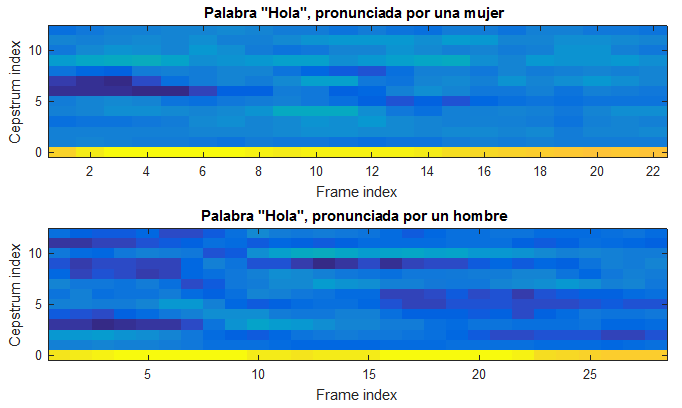
\includegraphics[width=0.8\linewidth]{figures/mfccHola}
			\caption{Palabra ``Hola' pronunciada por diferentes personas'.}
			\label{fig:ana:mfccHola}
	\end{figure}
	
	 \begin{figure}[H]
			\centering
			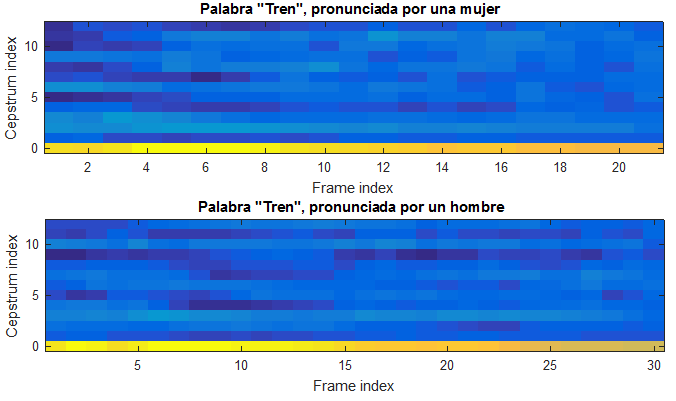
\includegraphics[width=0.8\linewidth]{figures/mfccTren}
			\caption{Palabra ``Tren'' pronunciada por diferentes personas.}
			\label{fig:ana:mfccTren}
	\end{figure}
	
	Y como complemento se propone el uso de cuantización vectorial debido al alto desempeño mostrado en \cite{A6}, \cite{A7} y \cite{A8}, además de que surge la necesidad de tener un tamaño fijo en los vectores de características ya que éstos serviran de entrada a la red neuronal que llevará a cabo el reconocimiento de las palabras, como se ve en las Figuras \ref{fig:ana:HolaRecorte}, \ref{fig:ana:mfccHola} y \ref{fig:ana:mfccTren} el índice se segmento varía, por lo que el número de coeficientes total depende de la duración de la muestra de voz.
	
	Finalmente, se opta por el uso de las redes neuronales, de acuerdo a los resultados obtenidos de \cite{A3} se propone el uso de una red neuronal \textit{feedforward} en su versión de \textit{Pattern Recognition Network} y para el entrenamiento se propone el uso del algoritmo \textit{Scaled Conjugate Gradient backpropagation} debido al alto desempeño que muestran en conjunto para reconocimiento de voz en señales con baja relación señal a ruido.

\subsection{Propuesta de frases}

Como propuesta inicial se plantea la obtención de las frases a reconocer de tres categorías de frases que corresponden a saludos, compras y la ciudad.

\paragraph{Saludos}\paragraph{}

Dentro de la costumbre mexicana, el saludo es un punto que hay que tener en cuenta, así como también los modales, es por eso que dentro de esta categoría se plantea el siguiente diccionario de palabras con las cuales se pueden formar diversos saludos y respuestas a éstos.

\begin{itemize}
\item	Buenos/Buenas: Se coloca una letra b sobre el corazón, y se mueve al frente.
\item	Hola: Se coloca una letra h sobre la frente, y se mueve hacia arriba.
\item	Días: se hace una d, y se mueve en medio círculo hacia un lado.
\item	Tardes: se coloca una t sobre el antebrazo, y se mueve en línea recta hacia usted.
\item	Noches: se coloca una g sobre la frente, y se mueve hacia abajo.
\end{itemize}

Así, de esta forma se cubren las frases básicas para esta categoría son:

 
\begin{table}[H]
\centering
\caption{Frases seleccionadas para la sección de saludos}
\label{tb:saludosFrases}
\begin{tabular}{|c|c|}
\hline
Hola, ¡buenos días!   & Hola, ¡buenas noches! \\ \hline
Hola, ¡buenas tardes! &                       \\ \hline
\end{tabular}
\end{table}
 
\paragraph{Compras}\paragraph{}

Uno de los aspectos cotidianos es el ir de compras, ya sea a la tienda o un súper mercado, esta categoría es extensa pues se pueden abordar diferentes tipos de compras, sin embargo, se tratará de una selección de frases que puedan ser usadas en cualquier sitio de compra. Estas frases fueron seleccionadas de una guía de frases en inglés haciendo referencia a compras. 

\begin{table}[H]
\centering
\caption{Frases seleccionadas para la sección de compras}
\label{tb:comprasFrases}
\begin{tabular}{|l|l|}
\hline
¿A qué hora abren?          & ¿Cuánto cuesta?          \\ \hline
¿A qué hora cierran?        & Estoy buscando (objeto), \\ \hline
¿Acepta tarjeta de crédito? & Me llevo esto.           \\ \hline
\end{tabular}
\end{table}
 
De este conjunto de frases se obtienen nuevas palabras que se reconocerán en el sistema

\paragraph{Ciudad}\paragraph{}

La tercera categoría abarca frases relacionadas con la ciudad, la utilidad de esta sección es para pedir informes dentro de la ciudad, así como también pedir indicaciones. Al igual que la categoría anterior, estas frases fueron seleccionadas de la misma guía anteriormente mencionada. 

\begin{table}[H]
\centering
\caption{Frases seleccionadas para la sección de ciudad}
\label{tb:ciudadFrases}
\begin{tabular}{|l|l|}
\hline
¿Disculpe, dónde está …?  & ¿Hay algún … cerca? \\ \hline
La oficina de información & Cajero              \\ \hline
La estación de autobuses  & Banco               \\ \hline
La estación de trenes     & Supermercado        \\ \hline
La estación de policía    & Farmacia            \\ \hline
                          & Metro               \\ \hline
                          & Hospital            \\ \hline
                          & Biblioteca          \\ \hline
\end{tabular}
\end{table}
 
Ya seleccionadas las frases con las que se trabajarán en la tabla 1 se presenta el listado general de palabras a reconocer.

\begin{table}[H]
\centering
\caption{Listado de palabras}
\label{tb:listadoPalabras}
\begin{tabular}{|l|l|l|}
\hline
\multicolumn{3}{|l|}{Listado de palabras por categoría} \\ \hline
Hola               & Estoy           & Estación         \\ \hline
Buenos/Buenas      & Buscando        & Autobuses        \\ \hline
Días               & Cuánto          & Trenes           \\ \hline
Tardes             & Cuesta          & Policía          \\ \hline
Noches             & Me              & Hay              \\ \hline
A                  & Llevo           & Algún            \\ \hline
Qué                & Esto            & Cerca            \\ \hline
Hora               & Disculpe        & Cajero           \\ \hline
Abren              & Dónde           & Banco            \\ \hline
Cierran            & Está            & Supermercado     \\ \hline
Acepta             & La              & Farmacia         \\ \hline
Tarjeta            & Oficina         & Metro            \\ \hline
De                 & Hospital        & Crédito          \\ \hline
Información        & Biblioteca      &                  \\ \hline
\end{tabular}
\end{table}


\subsection{Especificación de requisitos de software}

En esta sección se presenta la Especificación de Requisitos de Software (ERS) para la aplicación móvil que forma parte del proyecto terminal “Aplicación móvil para la comunicación con personas que utilizan el Lenguaje de Señas Mexicano (LSM)” según el estándar de IEEE 830.

%\subsubsection{Propósito}

%El propósito de este documento es definir la estructura y diseño de la aplicación móvil. Este documento va dirigido a toda persona interesada en el funcionamiento y estructuración del software a desarrollar.

\subsubsection{Ámbito del software}

\begin{itemize}
\item	La aplicación móvil llevará por nombre “Voice hands”.
\item	La aplicación interpretará un mensaje de voz a lenguaje de señas, representando el mensaje por medio de imágenes o animaciones.
\item	La aplicación no guardará los mensajes de voz.
\item	La aplicación contará con la capacidad de realizar síntesis de voz.
\item	No se podrán enviar mensajes digitales a través de la aplicación con otros usuarios.
\item	La aplicación permite la consulta de un diccionario del LSM por categorías.
\item	La aplicación reconocerá e interpretará cierta cantidad de frases limitadas por 43 palabras que se encuentran en el banco de reconocimiento.
\item	Con el desarrollo de esta aplicación se espera que las personas que utilizan el lenguaje de señas sean capaces de comunicarse con personas que no y a su vez, las personas que no hacen uso de éste sean capaces de comunicarse con personas que sí.
\item	Un beneficio de esta aplicación es que cualquier persona que cuente con un móvil Android podrá hacer uso de ella, sin hardware adicional.
\item	El objetivo de la aplicación móvil es lograr que las personas tengan mayor oportunidad de acercamiento a tecnologías que permitan realizar la comunicación sin hacer uso de hardware adicional.
\item	Se espera que el software en un futuro pueda ser capaz de admitir una ampliación a su vocabulario a reconocer.
\end{itemize}

\subsubsection{Del sistema}

\begin{itemize}
\item	La aplicación móvil tendrá conexión al servidor que llevará a cabo el procesamiento de voz y nos entregará el resultado, la conexión mediante Internet.
\item	El sistema permitirá el uso en cualquier momento.
\item	El sistema soportará diversas peticiones al mismo tiempo, el número de peticiones está por definirse de acuerdo a los algoritmos implementados.
\end{itemize}

\subsubsection{Visión general}

En las secciones siguientes se detalla la estructura y funcionamiento de la aplicación móvil, los requisitos del dispositivo que la ejecutará, diagramas de casos de uso, actividades y un esbozo general de la aplicación.

\subsubsection{Descripción general}
\paragraph{Perspectiva del producto}\paragraph{}

La aplicación móvil será totalmente independiente a cualquier otro producto, en un futuro la unión de dos aplicaciones no queda descartada, pues existen productos desarrollados y en desarrollo que contribuyen al proceso de comunicación con el uso del LSM y esta unión se podrá dar gracias a un content provider entre ambas aplicaciones. Para este trabajo se desarrollará la aplicación móvil que realice la traducción de un mensaje de voz a lenguaje de señas, se diseñará la aplicación móvil y desarrollará el sistema que permita el procesamiento de voz.

\paragraph{Funciones del producto}\paragraph{}

La aplicación móvil contará con tres funciones principales:

\begin{itemize}
\item	Traducción de voz a LSM: Esta función básicamente graba una frase en voz y la traduce a lenguaje de señas mexicana, mostrando el resultado mediante imágenes.
\item	Reproducción en voz de cualquier texto ingresado: Se toma el texto ingresado en un campo de texto y se realiza la síntesis en voz de éste.
\item	Consulta de un diccionario de LSM: Organizado por categorías, se podrán consultar palabras del LSM y la forma en que se realizan dichas señas.
\end{itemize}

\paragraph{Características de los usuarios}\paragraph{}

La aplicación móvil va dirigida a personas con interés de comunicarse principalmente con personas sordas que utilizan el LSM, además, también va dirigido a personas que utilizan el lenguaje de señas y que tienen interés en comunicarse con personas que no lo usan, estas personas deberán tener conocimiento básico del uso de aplicaciones móviles.

\paragraph{Restricciones y limitaciones}

El uso de esta aplicación se recomienda en dispositivos móviles con las siguientes características mínimas:
\begin{itemize}
\item	Smartphone Android versión 4.4.
\item	Memoria RAM de 1 GB.
\item	Memoria interna de 8 GB con memoria externa.
\item	CPU: Quad-core 1.4 GHz
\end{itemize}

Para el servidor que realizará el procesamiento:
\begin{itemize}
\item	Windows 8 o superior.
\item	Java 8 o superior.
\item	4 GB de memoria RAM.
\item	10 GB de disco duro disponibles.
\item	Procesador de doble núcleo a 1.8 GHz.
\item	MySQL server 5.6.
\end{itemize}

La aplicación será desarrollada en Android Studio versión 2.2 bajo el lenguaje de programación Java, el procesamiento de voz se llevará a cabo en un servidor con lenguaje C.

La comunicación con el servidor se llevará a cabo mediante web service a través del protocolo TCP/IP.

La aplicación móvil no contará con sistema de seguridad ya que no se estarán manejando datos delicados ni registro en ésta.

\paragraph{Suposiciones y dependencias}\paragraph{}

La aplicación móvil está diseñada para Android, si se desea migrar a otro sistema operativo se deberán revisar los requisitos del dispositivo, así como el cambio de desempeño e interfaces con el servidor, de igual forma, si el servidor se implementa en un sistema operativo, será necesario revisar la comunicación que se llevará a cabo con la aplicación móvil.

El número de palabras y/o frases en un futuro puede crecer, así que es posible que se requiera un servidor con mayor capacidad de procesamiento para llevar a cabo el reconocimiento de palabras.

\paragraph{Requisitos futuros}\paragraph{}

Las posibles mejoras a la aplicación serían la integración de un diccionario más amplio de reconocimiento, integración de un sistema de reconocimiento de imágenes para completar la comunicación bidireccional e incluir un curso sobre lenguaje de señas.

\subsubsection{Requisitos específicos}

\paragraph{Interfaces externas}

\begin{itemize}
\item	Ie1. La aplicación móvil tendrá una interfaz sencilla que permita al usuario intuir el funcionamiento y la sección de funciones de ésta.
\item	Ie2. La comunicación con el servidor se llevará a cabo mediante un web service a través del protocolo TCP-IP.
\item	Ie3. Para la realización de la función de \textit{text-to-speech} o síntesis de voz se hará uso de la API que Google nos proporciona.
\item	Ie4. El servidor utilizará el ODBC más adecuado  para comunicarse con la base de datos.
\end{itemize}

\paragraph{Funciones}
\begin{enumerate}[label=(\alph*)]
\item	Traductor de voz a LSM

\begin{itemize}
\item	Fa1. Se contará con un botón para iniciar la grabación de la voz. (Móvil)
\item	Fa2. Se enviará la voz o las características de ésta al servidor a través de un web service. (Móvil)
\item	Fa3. Se realizará el procesamiento de voz para determinar las palabras mencionadas. (Servidor)
\item	Fa4. Se mapeará la frase detectada con la estructura correspondiente al LSM. (Servidor)
\item	Fa5. Se leerá de la base de datos las imágenes o animaciones correspondientes a la frase detectada. (Servidor)
\item	Fa6. Se enviará a la aplicación móvil las imágenes o códigos de éstas para que en la pantalla muestre el mensaje con la estructura correcta. (Servidor)
\item	Fa7. La aplicación móvil mostrará en pantalla las imágenes o animaciones correspondientes a la frase mencionada.
\item	Fa8. El usuario sólo podrá decir frases cortas con duración no mayor a 10 segundos.
\end{itemize}

\item	Síntesis de voz a través del teclado

\begin{itemize}
\item	Fb1. El usuario a través del teclado en pantalla ingresa la frase a comunicar.
\item	Fb2. Haciendo uso de la API de Google de text to speech se realizará la síntesis del texto introducido.
\item	Fb3. El idioma soportado será el español de México.
\end{itemize}

\item	Diccionario del LSM

\begin{itemize}
\item	Fc1. El diccionario estará dividido por categorías.
\item	Fc2. Contará con filtros por categoría y un cuadro de búsqueda.
\item	Fc3. Al seleccionar la palabra, la aplicación le mostrará la imagen correspondiente, además de una breve descripción de su uso.
\end{itemize}

\end{enumerate}

Estas secciones serán alcanzables gracias a un menú lateral que nos ofrecerá la opción de ingresar a cada una.

\paragraph{Requisitos de rendimiento}
\begin{itemize}
\item	Rr1. La aplicación sólo podrá ejecutar una actividad a la vez, y será usada por un usuario.
\item	Rr2. La aplicación se conectará con el servidor que ejecutará el procesamiento de la voz.
\item	Rr3. El servidor tendrá la capacidad de atender a más de un usuario a la vez .
\item	Rr4. Se requiere que la aplicación cuente con conexión a Internet.
\item	Rr5. Dado el listado de palabras se plantea que la cantidad de registros almacenados en la base de datos sea en el orden de las decenas.
\end{itemize}

\paragraph{Restricciones de diseño}
\begin{itemize}
\item	Rd1. La interfaz de la aplicación móvil se desarrollará en Android Studio, haciendo uso de las formas ya establecidas.
\item	Rd2. La interfaz gráfica de la aplicación móvil se llevará a cabo siguiendo el diseño visual y de movimientos de la guía de Material Design para Android.
\item	Rd3. La interfaz será de fácil entendimiento para que todas las personas que lo deseen la puedan ocupar.
\item	Rd4. El servidor no contará con interfaz gráfica.
\item	Rd5. Se hará uso del diccionario “manos con voz” de María Serafín y Raúl González para la obtención de imágenes.
\end{itemize}

\paragraph{Atributos de la aplicación}
\begin{itemize}
\item	Aa1. La aplicación será diseñada para que pueda ser usada por todo tipo de personas.
\item	Aa2. No se requiere de un inicio de sesión, por lo que en un móvil pueden interactuar más personas.
\item	Aa3. Como trabajo a futuro serán ofrecidas las actualizaciones que permitan más características, así como también nuevas funciones.
\end{itemize}
